\section{Reprezentacje surowych danych}
\label{sec:raw-data-representations}

Obecny trend w dziedzinie przetwarzania języka migowego skupia się głównie na wizji komputerowej, gdzie do pewnego stopnia ograniczona jest semantyka języka. Dla transkrypcji języka migowego jednym z większych wyzwań jest etykietowanie danych oraz sposób przedstawienia danych wejściowych tak, aby były wzajemnie zrozumiałe bez utraty informacji.

\subsection{Nagrania wideo}
\label{subsec:video-recordings}

Najpowszechniejszą formą reprezentacji migowego w przestrzeni cyfrowej są filmy. Jest to najprostsza i bezpośrednia forma zapisu informacji, ale nie jest optymalna dla samego przetwarzania. Występuje przede wszystkim redundancja danych. Tło czy elementy ubioru nie mają żadnego znaczenia w dialogu, dlatego też tła przetwarzanych zestawów danych są często jednolite lub całkowicie wycięte. Treści dialogów migowych są anotowane za pomocą napisów czy też systemów notacji dla szerszego kontekstu przetwarzania. Takie dane można spotkać w korpusach języków migowych, choć nie zawsze kompletne. Z uwagi na różnice w semantyce, anotowana treść może być uogólniana. Usuwanie pojedynczych elementów w komunikacji, takich jak kierunek patrzenia czy zależności przestrzenne między sekwencjami znaków może znacznie wpłynąć na znaczenie przekazu. Szczególnie wtedy, gdy materiał jest przetwarzany znak po znaku~\cite{yin2020}.

Języki migowe nie są historycznie bogato udokumentowane tak jak języki mówione. W przeciwieństwie do języków fonicznych, języki migowe nie mają powszechnie przyjętej formy pisemnej, mimo że powstały różne systemy transkrypcji cheremów~\cite{stokoe1966}, które różnią się od siebie w zależności od regionu i szkoły dla niesłyszących, w której są nauczane. Problem stanowi też dostępność zbioru danych nawet do celów badawczych. Nie każdy zbiór danych jest publicznie dostępny i gotowy do pobrania w całości. Większość źródeł występuje w formie słownika, gdzie przeważnie możemy tylko wyszukać po jednym haśle. Rzadko kiedy jest dodatkowa informacja poza nagraniem. Na szczęście rozwijane są korpusy języków migowych. Tak jak korpusy języków mówionych mają zbiory tekstów, korpusy języków migowych zawierają wypowiedzi ludzi na nagraniach. Powstają dużo później niż dla języków fonicznych, a prace badawcze nad lingwistyką migową trwają od połowy zeszłego wieku. Chociażby dlatego, że są to bardzo młode języki. Sam polski język migowy istnieje jako jeden z najstarszych, a pierwsze wzmianki datują 200 lat wstecz~\cite{hollak1879}.

\subsection{Notacje wizualne}
\label{subsec:visual-notation}

Artykuł \enquote{Sign Language Structure: An Outline of the Visual Communication Systems of the American Deaf} Williama Stokoe jest jednym z najważniejszych publikacji w dziedzinie języków migowych, ponieważ stał się kamieniem milowym w badaniach lingwistyki migowej i przyczynił się do zmiany sposobu postrzegania tychże języków jako odrębnych i samodzielnych systemów językowych. Przedstawił w nim swoją teorię dotyczącą struktury języka migowego na przykładzie amerykańskiego języka migowego.

W artykule zaprezentował argumenty przeciwko dotychczasowym poglądom, według których język migowy był jedynie systemem symbolicznym, a nie językiem. Stokoe argumentował, że język migowy ma swoją unikalną gramatykę i leksykę, złożoną z reguł i struktur, które można badać tak samo, jak gramatykę języków mówionych. Autor przedstawił również nową metodę analizy języka migowego, opartą na zapisie gestów za pomocą symboli graficznych, co pozwoliło na badanie i opisywanie struktury języka migowego w sposób bardziej precyzyjny~\cite{stokoe2005}.

Pracownia Lingwistyki Migowej Uniwersytetu Warszawskiego w 2010 podjęła się stworzenia pierwszego korpusu polskiego języka migowego, a w ciągu 3 lat stał się największym zaanotowanym korpusem migowym na świecie~\cite{rutkowski2013}. Oprócz tłumaczenia filmów na język polski, do transkrypcji artykularnej została użyta notacja HamNoSys (Hamburg Sign Language Notation System)~\cite{hanke2004}. Jest to system transkrypcji fonetycznej znaków opracowany przez Uniwersytet Hamburski. Przewyższa on notację Stokoe pod względem struktury i możliwości ekspresji. Zaletą HamNoSys jest możliwość jednoznacznego opisu znaków przestrzeni trójwymiarowej.

Przykładowo dla słowa \enquote{inteligencja} notacja będzie \hampinchonetwo\hamextfingeru\hampalml\hamforehead\hamlrat\hamtouch\hamreplace\hamfingertwo\hamthumbopenmod, gdzie \hampinchonetwo\hamspace określa kształt ręki (złączony kciuk i wskazujący), a \hamextfingeru\hamspace kierunek prostego palca (góra) i \hampalml\hamspace skierowanie dłoni (lewo) w \hamforehead\hamlrat\hamtouch, czyli dotknięcie prawej części czoła. Ostatecznie \hamreplace\hamfingertwo\hamthumbopenmod\hamspace mówi nam, że zamieniony jest początkowy znak na wyprostowany palec wskazujący i odgięty kciuk.

\subsection{Szkieletowe modele sylwetki}
\label{subsec:skeletal-models}

W wizji komputerowej przestrzenne modele pozy są stosowane głównie przy szacowaniu lokalizacji postury człowieka na podstawie informacji z kamery, czujników inercyjnych, czy też kombinacji różnych sensorów.

Preferowanym modelem w ostatnich latach jest uproszczony model szkieletu człowieka o drzewiastej strukturze~\cite{dafnis2022}. Do detekcji lokalizacji części ciała największą skuteczność osiągają modele trenowane na sieciach konwolucyjnych. W efekcie możemy otrzymać pozycje stawów modelu szkieletowego lub nawet trójwymiarowe siatki pozy każdej klatki nagrania~\cite{choi2020}. W porównaniu do surowych nagrań wideo szkielet o wysokiej precyzji jest znacznie mniej złożony. Pozbywając się tekstur i kształtów, nie tracimy najważniejszych informacji do przetworzenia języka migowego. Poniżej przykład modelu na wybranych klatkach nagrania ze Słownika Korpusu Polskiego Języka Migowego~\cite{lacheta2016}.

\begin{figure}[H]
    \centering
    \begin{subfigure}{0.3\textwidth}
        \centering
        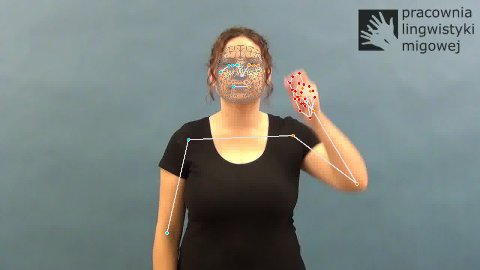
\includegraphics[width=\textwidth]{figures/intelligence-1}
        \caption{\hampinchonetwo\hamextfingeru}
        \label{fig:intelligence-1}
    \end{subfigure}
    \hfill
    \begin{subfigure}{0.3\textwidth}
        \centering
        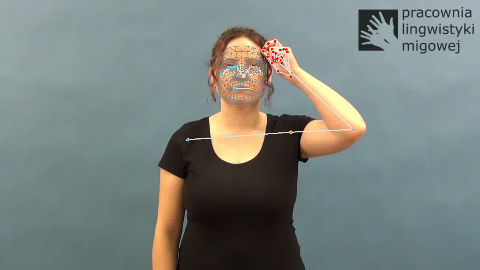
\includegraphics[width=\textwidth]{figures/intelligence-2}
        \caption{\hampalml\hamforehead\hamlrat\hamtouch}
        \label{fig:intelligence-2}
    \end{subfigure}
    \hfill
    \begin{subfigure}{0.3\textwidth}
        \centering
        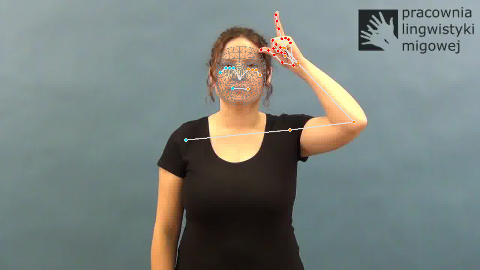
\includegraphics[width=\textwidth]{figures/intelligence-3}
        \caption{\hamreplace\hamfingertwo\hamthumbopenmod}
        \label{fig:intelligence-3}
    \end{subfigure}
    \caption{Model szkieletowy z siatką twarzy dla słowa \enquote{inteligencja}}
    \label{fig:intelligence}
\end{figure}
